\documentclass{article}
\usepackage[utf8]{inputenc}
\usepackage[ukrainian]{babel}
\PassOptionsToPackage{hyphens}{url}\usepackage{hyperref}
\title{Прикладні алгоритми. Завдання 2, звіт}
\author{Михайло Голуб}
\usepackage{graphicx}
\graphicspath{ {./images/} }
\begin{document}
\maketitle
\newpage

\textbf{Реалізація UnionFind:}\\\indent

Для зберігання інформації про належність елементу до множини створено клас Node з значеннями value, next та header.\\\indent
Для зберігання інформації про множину створено клас UnionFindSetMeta з значеннями head, tail, root та size, а також методами recalc\_size та recalc\_tail.\\\indent
Для реалізації структури UnionFind створено клас UnionFindHandler з наступною логікою роботи:
\begin{itemize}
\item існує словник універсуму, в якому знаходяться пари елемент-Node, елемент виступає ключем словника; 
\item метод make\_set додає нову пару з вказаним елементом, при цьому в класі Node міститься вказівник на відповідний UnionFindSetMeta;
\item метод find повертає корінь множини якій належить шуканий елемент, або -1 якщо його немає серед ключів словника;
\item метод union об'єднує дві множини до яких належать вказані елементи;
\item метод everything\_in\_one\_set повертає True якщо всі елементи містяться в одній множині, інакше -- False.
\end{itemize}


\textbf{Реалізація алгоритму Крускала:}\\\indent

З другого завдання імпортовано класи графів та класів що генерують випадкові графи. Алгоритм Крускала реалізовано наступним чином:
\begin{enumerate}
\item Алгоритм приймає на вхід зважений неорієнтований граф та видаляє з нього усі петлі;
\item Створюється масив усіх ребер: масив трійок значень (вага, вершина\_1, вершина\_2). При цьому кожна пара вершин опрацьовується лише один раз;
\item Масив усіх ребер сортується від найменшої ваги до найбільшої
\item Створюється зважений неорієнтований граф minimal\_tree з кількістю вершин рівною вхідному графу, але без ребер;
\item Створюється пуста структура UnionFind
\item Обрати неопрацьоване ребро з найменшою вагою;
\item Якщо обидві вершини відсутні в UnionFind -- додати їх туди та об'єднати їх в одну множину; запам'ятати ребро яке їх з'єднує;
\item Якщо одна з множин відсутня в UnionFind -- додати її туди та об'єднати з множиною якій належить інша вершина; запам'ятати ребро яке їх з'єднує;
\item Повторювати 6-8 доки не опрацьовані усі ребра, або "кількість вершин в універсумі рівна кількості вершин в графі та усі елементи UnionFind належать одній множині";
\item Записати в minimal\_tree усі запам'ятовані ребра та повернути його.
\end{enumerate}

\textbf{Аналіз часу роботи алгоритму Крускала:}\\\indent

В найгіршому випадку алгоритм Крускала має складність O(E*logV), де E це кількість ребер і V це кількість вершин. При подвоєнні вірогідності створення ребра очікуване подвоєння часу роботи. При збільшенні кількості вершин очікується спадання швидкості росту часу роботи. На тепловій карті нижче зображено залежність часу роботи алгоритму Крускала від кількості вершин у графі та ймовірності створення ребра.

\begin{center}
    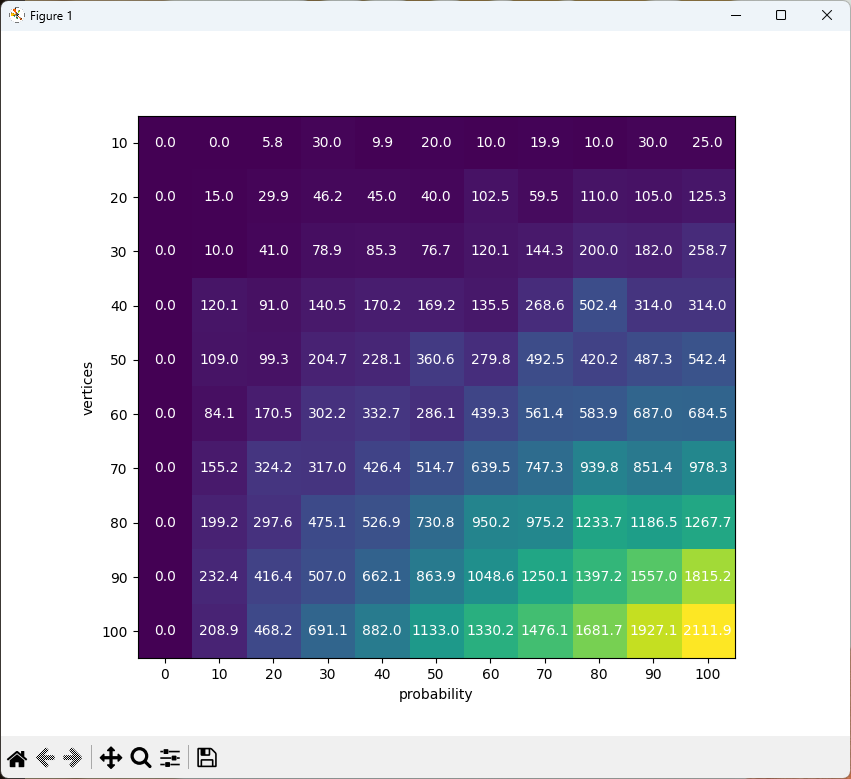
\includegraphics[width=125mm]{map}
\end{center}

З теплової карти видно, що колонки 10 та 20, 20 та 40, 30 та 60, 40 та 80 50 та 100 відрізняються приблизно в два рази, тож лінійну залежність від кількості ребер підтверджено.\\\indent

Для оцінки залежності часу роботи від кількості вершин було створено генератор випадкових графів з вказаною кількістю ребер. Десятки тестів на залежність часу роботи від кількості вершин при фіксованій кількості ребер не дали однозначного результату. Проведення тестів з високою кількістю повторів та великою кількістю досліджуваних кількостей вершин не є можливим, оскільки випадкова генерація великих графів, або малих графів у великій кількості, є дуже повільним процесом.\\\indent

Нижче наведено графік результатів одного з тестів. Як видно характер зростання експоненційний, хоч і має значний обчислювальний шум і дивне падіння на кількості вершин близько 800.

\begin{center}
    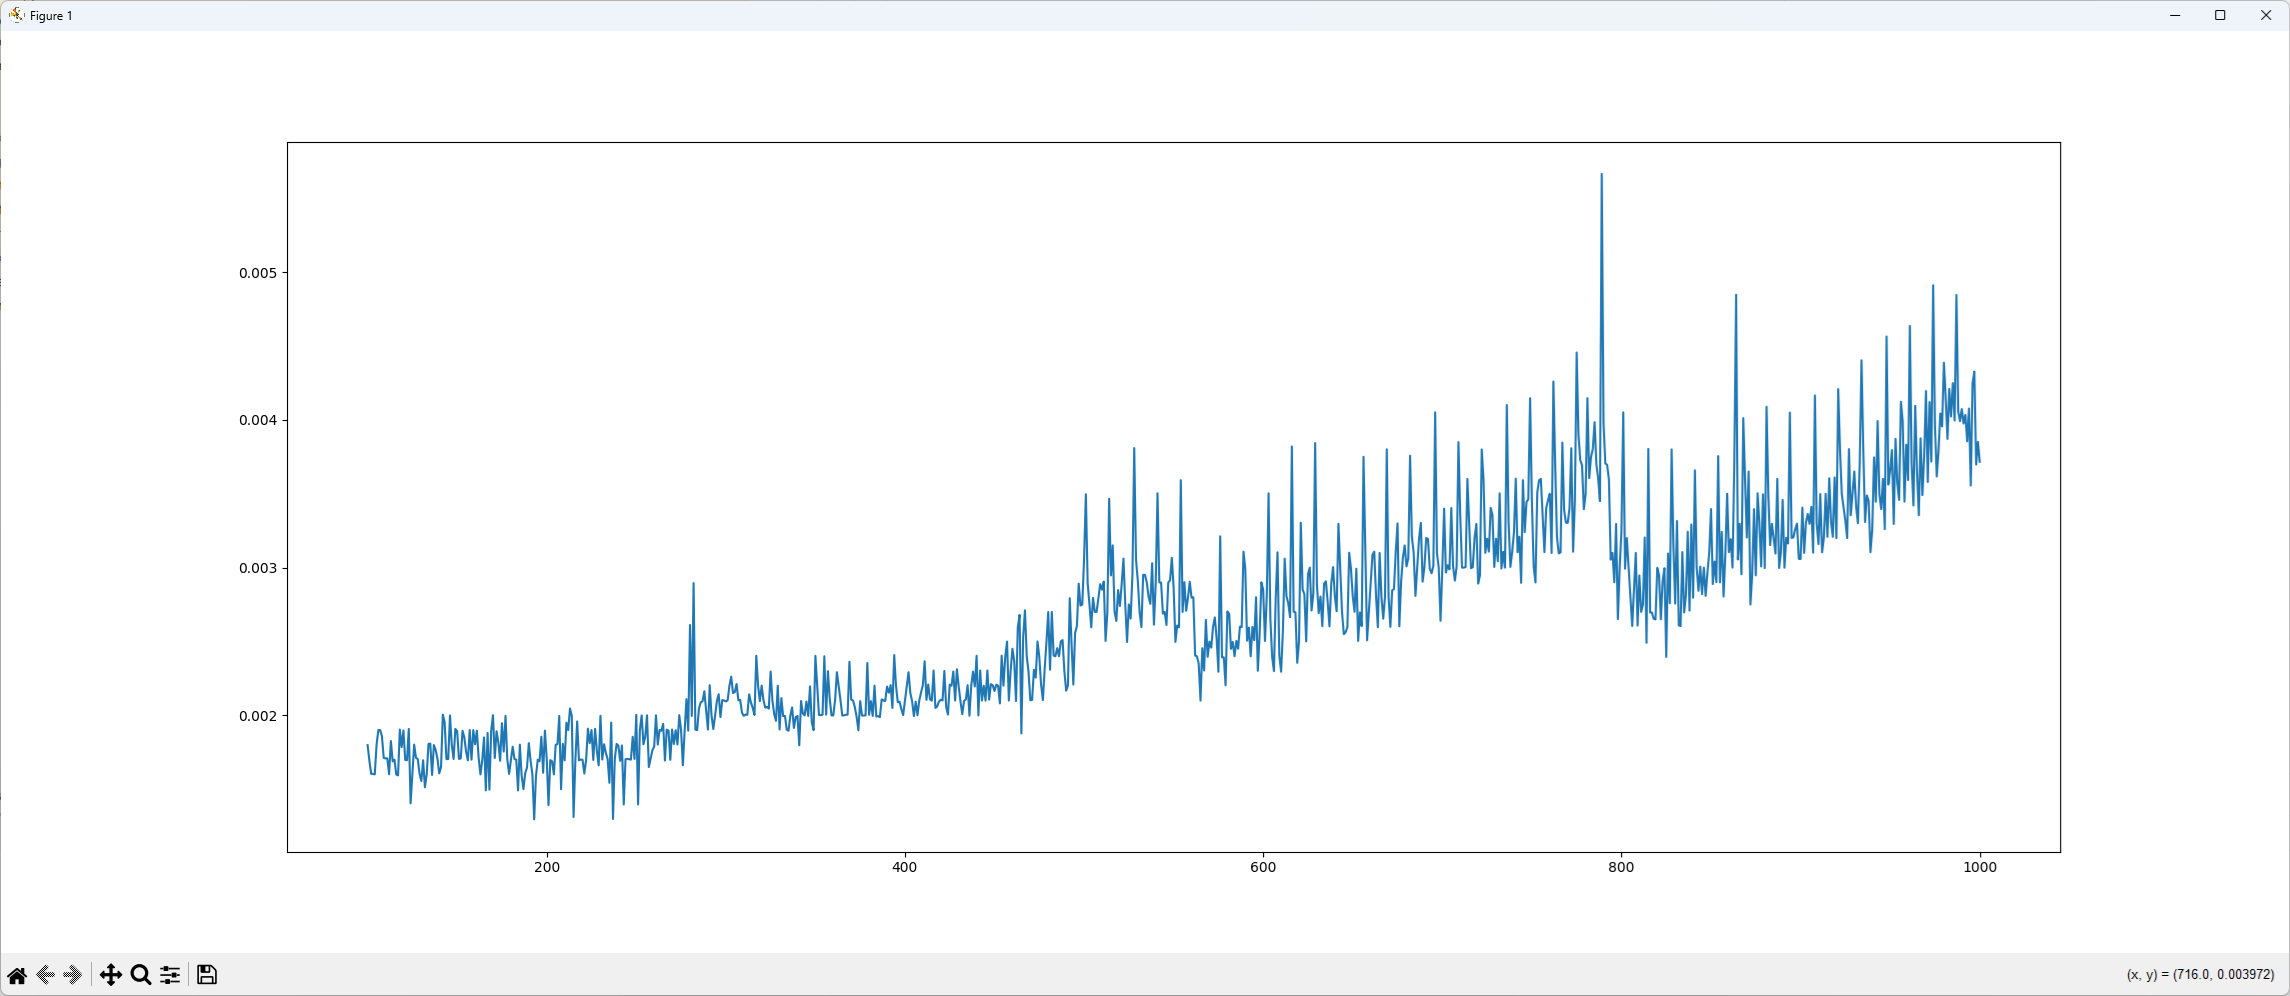
\includegraphics[width=125mm]{graph}
\end{center}

\textbf{Висновки:}\\\indent
\begin{itemize}
\item Структура UnionFind дуже зручна в роботі та швидкодійна, якщо немає потреби у видаленні елементів з множини;
\item Алгоритм Крускала можна реалізувати для раніше створених класів графів за допомогою структури UnionFind;
\item Час роботи алгоритму Крускала лінійно залежить від кількості ребер у графі, що збігається з теоретичною оцінкою;
\item Час роботи алгоритму Крускала скоріше за все експоненційно залежить від кількості вершин, що не збігається з теоретичною оцінкою.
\end{itemize}


Посилання на репозиторій практикуму:\\ \href{$https://github.com/MINIAProgramStudio/applied_algorythms/tree/main/task_4$}{$https://github.com/MINIAProgramStudio/applied\_algorythms/tree/main/task\_4$}
\end{document}